\documentclass[a4paper,11pt]{article}

\usepackage[utf8]{inputenc}

\usepackage{amssymb}
\usepackage{enumerate}%\usepackage{paralist}
\usepackage{bm}%bold math
\usepackage{amsmath}%math formulas
\usepackage{amsthm}%ems,Proofs
\usepackage{yhmath}%dots
\usepackage{fontenc}
\usepackage{wasysym}%Various math symbols
\usepackage{MnSymbol}
\usepackage{color}
\usepackage{array}
\usepackage{ragged2e}
\usepackage{epstopdf}
\usepackage{graphicx} % Allows including images
\usepackage{xcolor}
\usepackage{booktabs}
%% Define a new command as Steven B. Segletes suggested:
\newcommand*{\lrrule}[1]{\hrulefill\hspace*{2.5mm}\raisebox{-.3\ht\strutbox}{#1}\hspace*{2.5mm}\hrulefill}

\definecolor{babyblue}{HTML}{4591CD}

\newcommand\gre\relax
\newcommand\eng\relax
\begin{document}
\begin{center}
	\begin{minipage}{0.1\textwidth}
				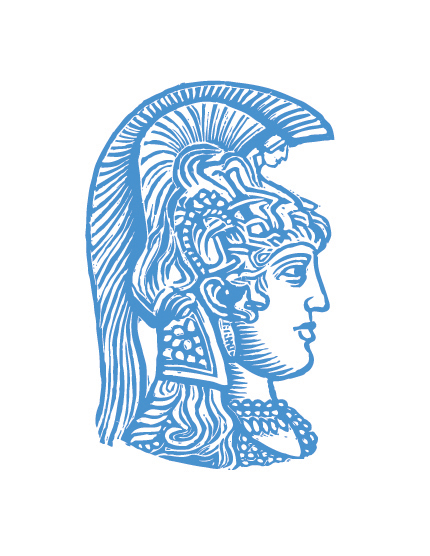
\includegraphics[scale=0.5]{/Users/giannistsagaropoulos/Documents/Πανεπιστήμιο/2ο-Εξάμηνο/Πληροφορική-ΙΙ/Exercises/Εργασία_2/Figures/ekpa_logo.jpg}
			\end{minipage}
			\begin{minipage}{0.40\textwidth}
				\centering
				\footnotesize{\textrm{HELLENIC REPUBLIC}}\\
				\scriptsize{\textbf{\textrm{National and Kapodistrian}\\\textrm{University of Athens}}}\\
				\vspace{1.5mm}
				{\color{babyblue} 
				\rule[0.7mm]{8.5mm}{0.17mm} \tiny{\textrm{EST. 1837 }}\rule[0.7mm]{9.5mm}{0.17mm}
				}%\\[2mm]
			\end{minipage}

%% Change the width of the box.
%\ruletext[5cm]{\textbf{FOUNDED IN 1837}}
\end{center}

{\color{babyblue} \rule[0cm]{5mm}{0.2mm} asdfsa}
\end{document}
